\documentclass[english]{article}
%\usepackage{color}
\usepackage{verbatim}
\usepackage{amssymb}
\usepackage{amsmath}
\usepackage{amsfonts}
\usepackage{amsthm}
\usepackage{graphicx}

%%%%%%%%%%%%%%%%%%%%%%%%%%%%%% Textclass specific LaTeX commands.
\theoremstyle{plain}
\newtheorem{thm}{\protect\theoremname}
  \theoremstyle{plain}
  \newtheorem{lem}[thm]{\protect\lemmaname}

%%%%%%%%%%%%%%%%%%%%%%%%%%%%%% User specified LaTeX commands.

%%--- icml specific ------

% As of 2011, we use the hyperref package to produce hyperlinks in the
% resulting PDF.  If this breaks your system, please commend out the
% following usepackage line and replace \usepackage{icml2015} with
% \usepackage[nohyperref]{icml2015} above.
%\usepackage{hyperref}

% Packages hyperref and algorithmic misbehave sometimes.  We can fix
% this with the following command.
\newcommand{\theHalgorithm}{\arabic{algorithm}}
% icml template 

\usepackage[accepted]{icml2015}

% The \icmltitle you define below is probably too long as a header.
% Therefore, a short form for the running title is supplied here:
%\icmltitlerunning{Kernel-Based Just-In-Time Learning for Passing Expectation Propagation Messages}
\icmltitlerunning{ Just-In-Time Kernel Regression for Expectation Propagation }
%% ---- end icml specific ----

\usepackage{algorithmic}
\usepackage{algorithm}

\renewcommand{\algorithmicrequire}{\textbf{Input:}}
\renewcommand{\algorithmicensure}{\textbf{Output:}}

\usepackage{appendix}
\usepackage{natbib}
\usepackage{soul}
\usepackage{subfig}
\usepackage{times}

% \usepackage{tikz}
% \usetikzlibrary{bayesnet}

\usepackage[textsize=small]{todonotes}

\usepackage{url}


\newcommand{\diag}{\mathop{\mathrm{diag}}}
\newcommand{\trace}{\mathop{\mathrm{tr}}}
\newcommand{\median}{\mathop{\mathrm{median}}}

\newcommand{\bx}{\mathbf{x}}				% all variables
%\newcommand{\factor}{\psi}				% factor
\newcommand{\factor}{f}				% AG: made this f for consistency
\newcommand{\outV}{V}                         %AG: output variable of a factor
\newcommand{\fis}[1]{\mathrm{ne}(#1)}   	% index set for variables connected to  factor
\newcommand{\fx}[1]{ \mathbf{x}_{\mathrm{ne}(#1)} }   	% variables of a factor
\newcommand{\xin}{\mathbf{x}_{ \mathrm{in} }} 			% parents of directed factor
\newcommand{\xout}{\mathbf{x}_{ \mathrm{out} }}			% child of directed factor
\newcommand{\msg}[2]{m_{#1 \rightarrow #2}}			% message from arg1 to arg2
\newcommand{\approxMsg}[3]{M_{#1 \rightarrow #2}^{#3}}			% message from arg1 to arg2
\newcommand{\uncert}{{\mathfrak v}}          %%AG: variable used to denote uncertainty
\newcommand{\uncertaintyMsg}[3]{{\mathfrak V}_{#1 \rightarrow #2}^{#3}}			% message from arg1 to arg2
\newcommand{\diffd}{\mathrm{d}}
%\newcommand{\proj}{\mathrm{proj}}   %AG: replaced with notation using less space

%\newcommand{\proj}{\mathbb{Q}}


\newcommand{\projP}[1]{\mathrm{proj} \left [ #1 \right]}   
%\newcommand{\projP}[1]{\mathbb{Q} \left [ #1 \right]} %AG: replaced with notation using less space
\DeclareMathOperator*{\proj}{\text{proj}} % WJ defined this

\newcommand{\argmin}[1]{\mathrm{arg}\mathrm{min}_{#1}}
\newcommand{\kld}[2]{\mathrm{KL} \left [ #1 || #2 \right ]}
\newcommand{\expectationE}[2]{ \mathbb{E}_{#2}  \left[ #1 \right] }

% random features stuff
\newcommand{\feax}{\mathsf{x}}
\newcommand{\feaX}{\mathsf{X}}
\newcommand{\feay}{\mathsf{y}}
\newcommand{\feaY}{\mathsf{Y}}

% \newcommand{\wjnote}[1]{\textbf{\color{blue!90!black}{WJ: #1}}  }
% \newcommand{\aenote}[1]{\textbf{\color{red!50!black}{#1}} }
% \newcommand{\nhnote}[1]{\textbf{\color{magenta!90!black}{#1}} }
% \newcommand{\agnote}[1]{\textbf{\color{green!50!black}{#1}} }
% \newcommand{\dsnote}[1]{}%\textbf{\color{orange!50!black}{#1}} }
\newcommand{\wjnote}[1]{ }
\newcommand{\aenote}[1]{}
\newcommand{\nhnote}[1]{}
\newcommand{\agnote}[1]{}
 \newcommand{\dsnote}[1]{}%\textbf{\color{orange!50!black}{#1}} }

\newcommand{\figref}[1]{Fig.~\ref{#1}}
\newcommand{\secref}[1]{Section~\ref{#1}}
\newcommand{\tabref}[1]{Table.~\ref{#1}}
%\newcommand{\eqref}[1]{Eq.~\ref{#1}}


%\makeatother

\usepackage{babel}
  \providecommand{\lemmaname}{Lemma}
\providecommand{\theoremname}{Theorem}


% WJ's space hacks. 
\setlength{\intextsep}{2mm}
\setlength{\dbltextfloatsep }{2mm}
\setlength{\dblfloatsep}{4mm}
\setlength{\belowcaptionskip}{1mm}
\setlength{\abovecaptionskip}{2mm}

% \floatsep: space left between floats.
% \textfloatsep: space between last top float or first bottom float and the text.
% \intextsep : space left on top and bottom of an in-text float.
% \dbltextfloatsep is \textfloatsep for 2 column output.
% \dblfloatsep is \floatsep for 2 column output.
% \abovecaptionskip: space above caption
% \belowcaptionskip: space below caption
\tolerance 1414
\hbadness 1414
\emergencystretch 1.5em
\hfuzz 0.3pt
\widowpenalty=10000
\vfuzz \hfuzz
\raggedbottom
\graphicspath{{../uai2015/img/}}


\begin{document}

\twocolumn[
%\icmltitle{Kernel-Based Just-In-Time Learning for \\Passing Expectation Propagation Messages}
\icmltitle{Just-In-Time Kernel Regression for Expectation Propagation}

\icmlauthor{Wittawat Jitkrittum$^*$}{wittawatj@gmail.com}
\icmlauthor{Arthur Gretton$^*$}{arthur.gretton@gmail.com}
\icmlauthor{Nicolas Heess}{nheess@nhuk.de}
\icmlauthor{S. M. Ali Eslami}{ali@arkitus.com}
\icmlauthor{Balaji Lakshminarayanan$^*$}{balaji@gatsby.ucl.ac.uk}
\icmlauthor{Dino Sejdinovic$^\dagger$}{dino.sejdinovic@gmail.com}
\icmlauthor{Zolt{\'a}n Szab{\'o}$^*$}{z.szabo@ucl.ac.uk}

\icmladdress{$^*$Gatsby Unit, University College London}
\vspace*{-3mm}
\icmladdress{$^\dagger$University of Oxford}

\icmlkeywords{expectation propagation, kernel, online learning, mean embedding, random features}

]

%\title{Kernel-Based Just-In-Time Learning for \\Passing Expectation Propagation
%Messages}

%\author{
%Wittawat Jitkrittum$^1$, \, Arthur Gretton$^1$, \, Nicolas Heess, \, \textbf{S. M. Ali Eslami} \\
%\textbf{Balaji Lakshminarayanan}$^1$, \, \textbf{Dino Sejdinovic}$^2$ \and \textbf{ Zolt{\'a}n Szab{\'o}}$^1$  \vspace*{2mm} \\
%Gatsby Unit, University College London$^1$ \\
%\vspace*{2mm}
%University of Oxford$^2$ \\
%\texttt{ \{wittawatj,  arthur.gretton\}@gmail.com}, \, \texttt{nheess@nhuk.de} \\ 
%\texttt{ali@arkitus.com}, \, \texttt{balaji@gatsby.ucl.ac.uk},\\
%\texttt{dino.sejdinovic@gmail.com},\, \texttt{z.szabo@ucl.ac.uk}
%}
%\maketitle



\begin{abstract}

We propose an efficient nonparametric strategy for learning a message operator in expectation propagation (EP), which takes as input the set of incoming messages to a factor node, and produces an outgoing message as output. This learned operator replaces the multivariate integral required in classical EP, which may not have an analytic expression. We use kernel-based regression, which is trained on a set of probability distributions representing the incoming messages, and the associated outgoing messages. The kernel approach has two main advantages: first, it is fast, as it is implemented using a novel two-layer random feature representation of the input message distributions; second, it has principled uncertainty estimates, and can be cheaply updated online, meaning it can request and incorporate new training data when it encounters inputs on which it is uncertain.  In experiments, our approach is able to solve learning problems where a single message operator is required for multiple, substantially different data sets (logistic regression for a variety of classification problems), where the ability to accurately assess uncertainty and to efficiently and robustly update the message operator are essential.

\end{abstract}


\section{Introduction}


An increasing priority in Bayesian modelling is to make inference accessible and implementable for practitioners,
without  requiring specialist knowledge.
% in Bayesian inference.
This
is a goal sought in probabilistic programming languages \citep{WinGooStuSis11,GooManRoyBonTen08}, 
as well as in more granular, component-based
systems \citep{SDT2014,Minka2014}. In all cases, the user
should be able to freely specify what they wish their model to express,
without having to deal with the complexities of sampling, variational
approximation, or distribution conjugacy.  In reality, however, model convenience and
simplicity can  limit
or undermine intended models, sometimes in ways the users
might not expect. 
%To take one example, the inverse gamma prior, which is
%widely used due to being a convenient
%conjugate prior for the variance, has quite pathological behaviour \citep{Gelman2006}.
In general, more expressive, freely chosen models are more likely
to require expensive sampling or quadrature approaches, which can make
them challenging to implement or impractical to run.

In this work, we address the particular setting of expectation propagation 
\citep[EP;][]{Minka2001}, a message passing algorithm wherein messages are confined to
being members of a particular parametric family. Sending EP outgoing messages
requires an expensive computation involving integrating incoming messages over a
factor potential, and projecting the result onto the chosen family. We propose
a novel, kernel-based approach to learning a message operator nonparametrically
for EP. The learning algorithm takes the form of a
distribution regression problem, where the inputs are probability measures (incoming messages), and
the outputs are vectors of message parameters \citep{Szabo2014}.  

Being an instance of Gaussian process regression, there are well established
estimates of predictive uncertainty \citep[Ch. 2]{RasWil06}.  We use these
uncertainty estimates to determine when to query the importance sampler for
additional input/output pairs.  To make the algorithm computationally
tractable, we regress  directly in the primal from random Fourier features of
the data \citep{Rahimi2007,Le2013,YanSmoZonWil14}.  In particular, we establish
a novel random feature representation for when inputs are distributions, via a
two-level random feature approach.

%%%%%%%%%%%%%%%%%%%%%%%%%%%%%%%%%%%%%%%%%%%%%%%%%%%%%%%%%%%%%%%%%%%%%%%%%%%%%%%%%%%%%%%%%%



\section{Background}
\label{sec:EP}

We assume that distributions (or densities) $p$ over a set of variables 
$\bx = (x_1, \dots x_d)$ of interest can be represented as factor graphs, i.e.\
%
%\begin{equation*}
$p(\bx) = \frac{1}{Z} \prod_{j=1}^J \factor_j(\fx{\factor_j})$.
%\end{equation*}
The factors $\factor_j$ are non-negative functions which are defined over subsets $\fx{\factor_j}$ of the full set of variables $\bx$. These variables form the neighbors of the factor node $\factor_j$ in the factor graph, and we use $\fis{\factor_j}$ to denote the corresponding set of indices. $Z$ is the normalization constant.

We deal with models in which some of the factors have a non-standard form, or
may not have a known analytic expression (i.e.\ ``black box'' factors).
Although our approach applies to any such factor in principle, in this paper we
focus on \textit{directed} factors $\factor(\xout | \xin)$ which specify a
conditional distribution over variables $\xout$ given $\xin$ (and thus
$\fx{\factor} = (\xout, \xin))$. The only assumption we make is that we are
provided with a forward sampling function $f: \xin \mapsto \xout$. 
In particular, the ability to evaluate the value of $\factor(\xout | \xin)$ is
not assumed.


%--------------------------------------------------------------------

\subsection{Expectation propagation}
\label{sec:EP:MP}

%AG: I like this explanation,but we are short of space, so I am commenting it out.
%Belief propagation -- or the sum-product algorithm -- computes marginal distributions over subsets of variables by iteratively passing messages between variables and factors, ensuring consistency of the obtained marginals at convergence. Specifically, the messages sent from a factor $\factor$ to variable $x_i$ (where $i \in \fis{\factor}$) are computed as
%\begin{equation}
%\msg{ \factor }{i}(x_i) = 
%\int \factor (\fx{\factor}) \prod_{i' \in \fis{\factor} \textbackslash i} \msg{i'}{\factor}(x_{i'}) \diffd \bx_{\fis{\factor} \textbackslash i},
%\label{eq:msgPassing:BP}
%\end{equation}
%where $\msg{i'}{\factor}$ are the messages sent to factor $\factor$ from its neighboring variables $x_{i'}$ other than $x_i$.

Expectation Propagation (EP) is an approximate iterative procedure for
computing marginal beliefs of variables by iteratively passing messages between
variables and factors until convergence \citep{Minka2001}.  The message $\msg{
\factor }{\outV}(x_{\outV})$  from factor $\factor$ to variable
$\outV\in\fis{\factor}$ is 
%
\begin{equation}
% \frac{ \projP{ \msg{\outV}{\factor}(x_{\outV})
% \int \factor (\fx{\factor}) \prod_{\outV'} \msg{\outV'}{\factor}(x_{\outV'}) \diffd \bx_{\fis{\factor} \textbackslash \outV}} }
% {\msg{\outV}{\factor}(x_{\outV})}
\frac{ \projP{ 
\int \factor (\fx{\factor}) \prod_{\outV' \in \fis{\factor}} \msg{\outV'}{\factor}(x_{\outV'}) \diffd 
\bx_{\fis{\factor} \backslash \outV}} }
{\msg{\outV}{\factor}(x_{\outV})}
%
\label{eq:msgPassing:EP}
\end{equation}
%
where $\msg{\outV'}{\factor}$ are the messages sent to factor $\factor$ from all of its neighboring variables $x_{\outV'}$,
%other than $x_{\outV}$,  
$\projP{p} = \argmin{q \in \mathcal{Q}} \kld{p}{q}$, and $\mathcal{Q}$ is in the exponential family.
%--------------------------------------------------------------------

%\subsection{Monte-Carlo message approximation}
%\label{sec:EP:MC}

%By projecting messages onto simple parametric forms, EP introduces an approximation that allows message passing to proceed when the true messages are not easily representable in closed form.
Computing the numerator of (\ref{eq:msgPassing:EP}) can be challenging and
often requires hand-crafted approximations, or
the use of expensive numerical integration techniques; for ``black-box''
factors $\factor$ implemented as forward sampling functions, fully
nonparametric techniques are needed. 
\citet{Barthelme2011,Heess2013,Eslami2014} propose an alternative
approach to the integration and projection step based on the following well known result.  
When the projection $\proj$
is to a member $q(x|\eta)=h(x)\exp\left(\eta^{\top}u(x)-A(\eta)\right)$ of an
exponential family, one simply computes the expectation of the sufficient
statistic $u(\cdot)$ under the numerator of (\ref{eq:msgPassing:EP}).
The estimated expected sufficient statistics provide us with an estimate
of the parameters $\eta$ of the result $q$ of the projection $\projP{p}$, from
which the message is readily computed.\dsnote{isn't $\eta$ the actual message?}


%--------------------------------------------------------------------

\subsection{Learning to pass EP messages}
\label{sec:EP:JIT}

One approach to compute the expected sufficient statistics, due to \citet{Barthelme2011}, is 
via importance sampling.  While these estimates converge to the desired
integrals for a sufficient number of importance samples, the sampling procedure
must be run at every iteration during inference, hence  it is not viable for
large-scale problems.

An improvement on this approach is to use importance sampled instances of input/output
message pairs to train a regression algorithm, which can then be used in place of the sampler.
\citet{Heess2013} use a neural network to learn the mapping from incoming
to outgoing messages. Specifically, they trained 
a neural network to directly map $(\msg{\outV'}{\factor} )_{\outV'
    \in \fis{\factor}}$ to 
    $\msg{\factor}{\outV}$, i.e.\ they learn a mapping
\begin{equation}
\approxMsg{\factor}{\outV}{\theta}: (\msg{\outV'}{\factor} )_{\outV' \in \fis{\factor}} \mapsto \msg{\factor}{\outV},
\end{equation}
where $\theta$ are the parameters of the approximator.

Although the learned mappings perform well on a variety of practical problems, 
this approach comes with a disadvantage: it requires training data
that cover the entire set of possible input messages for a given type of problem (e.g., datasets
representative of all classification problems the user proposes to solve),
and it has no way of assessing the uncertainty of its prediction, or of updating
the model online in the event that a prediction is uncertain.


The disadvantages of the neural network approach were the basis for work by
\citet{Eslami2014}, who replaced the neural networks with random forests.
The random forests  provided uncertainty estimates for each prediction. This
allowed them to be trained `just-in-time', during EP inference, whenever the
predictor decided it was uncertain. That is, if the uncertainty on the current
input messages exceeds a pre-defined threshold, the required outgoing message
is approximated via importance sampling  and
$\approxMsg{\factor}{\outV}{\theta}$ is updated on this new data point (leading
to a new set of parameters  $\theta'$). 
However, uncertainty estimation for random forests relies on unproven
heuristics: such heuristics can become highly misleading as we move away from
the training data.


%=============================================
\section{Kernel learning of operators}\label{sec:Online}
%=============================================

We now propose a kernel regression method for jointly learning the message operator $\approxMsg{\factor}{\outV}{\theta}$ and
uncertainty estimate. We will regress from the tuple of incoming messages, which
are probability distributions, to the parameters of the outgoing message. 

%------------------------------------
\subsection{Kernels on tuples of distributions}\label{sec:kernelsOnDistributions}
%------------------------------------

In contrast to \citet{Eslami2014,Heess2013} our kernel-based approach does not
need a pre-specified customized features to represent incoming messages.
Rather, we use a general characteristic kernel operated directly on distributions
\citep[eq.  9]{Christmann2010}.

In the following, we consider only a single factor, and therefore drop the factor identity from our notation. We write the set of $c$ incoming messages to a factor node as a tuple of
probability distributions %$\mathsf{x}_r:=$
$R:=(r^{(l)})_{l=1}^c$ of random variables $X^{(l)}$ on respective  domains $\mathcal{X}^{(l)}$.
Our goal is to define a kernel between one such tuple, and a second one,
which we will write %$\mathsf{x}_s:=$
$S:=(s^{(l)})_{l=1}^c$.

We define our kernel in terms of embeddings of the tuples $R,S$ into a reproducing kernel Hilbert space (RKHS). We first consider the embedding of a single distribution
in the tuple: Let us define a RKHS
$\mathcal{H}^{(l)}$ on each domain, with respective kernels $k^{(l)}(x^{(l)}_1,x^{(l)}_2)$.
We may embed individual probability distributions to these RKHSs, following \citet{Smola2007}.
The {\em mean embedding} of $r^{(l)}$ is written
$\mu_{r^{(l)}}(\cdot) := \int k^{(l)}(x^{(l)},\cdot) \, dr^{(l)} (x^{(l)})$,
such that
$\langle f,\mu_{r^{(l)}} \rangle_{\mathcal{H}^{(l)}} = \mathbb{E}_{r^{(l)}}(f(X^{(l)})), $ for all $f\in \mathcal{H}^{(l)}$.
%
Similarly, a mean embedding may be defined on the product of  messages in a tuple
$\mathsf{r}=\times_{l=1}^{c}r^{(l)}$ as
%
\begin{equation}
\mu_{\mathsf{r}}
:=
%\int k([x^{(1)} \hdots x^{(c)}],\cdot) \prod_{l=1}^{c}dr^{(l)}(x^{(l)}),
\int k([x^{(1)}, \ldots, x^{(c)}],\cdot) \, d\mathsf{r}(x^{(1)}, \ldots, x^{(c)}),
\label{eq:featureOfTuple}
\end{equation}
where we have defined the joint kernel $k$ on the product space
%concatenation of the features
$\mathcal{X}^{(1)}\times\cdots\times\mathcal{X}^{(c)}$.
Finally,  a kernel on two such embeddings $\mu_{\mathsf{r}},\mu_{\mathsf{s}}$ of tuples $R,S$ can be obtained as in \citet[eq. 9]{Christmann2010}:
%
\begin{equation}
\kappa(\mathsf{r}, \mathsf{s}) = \exp\left(-\frac{\|\mu_{\mathsf{r}}-\mu_{\mathsf{s}}\|_{\mathcal{H}}^{2}}{2\gamma^{2}}\right).
\label{eq:gauss_joint_emb}
\end{equation}
%
This kernel has two parameters: $\gamma^{2}$, and the width parameter of the kernel $k$ defining $\mu_{\mathsf{r}} = \mathbb{E}_{\mathsf{r}}k(x,\cdot)$.



%------------------------------------
\subsection{Random feature approximations}
%------------------------------------
\label{sec:randomFeatureApproximations}

\begin{algorithm}[t]
\caption{Construction of two-stage random features for $\kappa$}
\label{algo:random_features_kgg}
\begin{algorithmic}[1]
\REQUIRE Input distribution $\mathsf{r}$, Fourier transform $\hat{k}$ of 
the embedding translation-invariant kernel $k$, number of inner features $D_\mathrm{in}$, number of outer features $D_\mathrm{out}$, outer Gaussian width $\gamma^2$.
\ENSURE Random features $\hat{\psi}(\mathsf{r}) \in \mathbb{R}^{D_\mathrm{out}}$. 

%\STATE Compute the Fourier transform $\hat{k}$ of the kernel $k$.
\STATE Sample  $\{ \omega_i \}_{i=1}^{D_\mathrm{in}} \overset{i.i.d}{\sim} \hat{k}$.
\STATE Sample $\{b_i\}_{i=1}^{D_\mathrm{in}} \overset{i.i.d}{\sim} \text{Uniform}[0, 2\pi] $.
\STATE $\hat{\phi}(\mathsf{r}) = \sqrt{\frac{2}{D_\mathrm{in}}} \left( \mathbb{E}_{\mathsf{r(x)}} 
\cos(\omega_{i}^{\top}x+b_{i} ) \right)_{i=1}^{D_\mathrm{in}} \in \mathbb{R}^{D_\mathrm{in}}$ \\
%\STATE  $\hat{\phi}(p)=\mathbb{E}_{p(x)}\sqrt{\frac{2}{D_\mathrm{in}}}\left(\cos\left(\omega_{1}^{\top}x+b_{1}\right),\ldots,\cos\left(\omega_{D_\mathrm{in}}^{\top}x+b_{D_\mathrm{in}}\right)\right)^{\top}$.
If $\mathsf{r}(x)=\mathcal{N}(x;m, \Sigma )$, 
\small
\begin{equation*}
\hat{\phi}( \mathsf{r}) = \sqrt{\frac{2}{D_\mathrm{in}}} \left( \cos(\omega_{i}^{\top}m +b_{i}) \exp 
\left(-\frac{1}{2}\omega_{i}^{\top}\Sigma \omega_{i} \right) \right)_{i=1}^{D_\mathrm{in}}.
\end{equation*}
%Even if $p$ is not a normal distribution, we may still use it as an approximation.
%
\STATE Sample $\{ \nu_i \}_{i=1}^{D_\mathrm{out}} \overset{i.i.d}{\sim} \hat{k}_{\text{gauss}}(\gamma^{2})$.  
i.e., Fourier transform of a Gaussian kernel with width $\gamma^2$.
\STATE Sample $\{c_i\}_{i=1}^{D_\mathrm{out}} \overset{i.i.d}{\sim} \text{Uniform}[0, 2\pi] $.
\STATE $\hat{\psi}(\mathsf{r}) = \sqrt{\frac{2}{D_\mathrm{out}}} \left(  
\cos(\nu_{i}^{\top} \hat{\phi}(\mathsf{r}) + c_{i} ) \right)_{i=1}^{D_\mathrm{out}} \in 
\mathbb{R}^{D_\mathrm{out}}$
\end{algorithmic}
\end{algorithm}
%AG: replaced ``kernel ridge'' wiht Gaussian process'' so as not to switch back and forth.

One approach to learning the mapping  $\approxMsg{\factor}{\outV}{\theta}$ from incoming to outgoing messages
would be to employ Gaussian process regression, using the kernel \eqref{eq:gauss_joint_emb}.
This approach is not suited to just-in-time (JIT) learning, however,
as both prediction and storage cost grow with the size of the training set.
Instead, we define 
a finite-dimensional random feature map $\hat{\psi} \in \mathbb{R}^{D_\mathrm{out}}$ such that 
$\kappa(\mathsf{r}, \mathsf{s}) \approx \hat{\psi}(\mathsf{r})^\top \hat{\psi}(\mathsf{s})$, 
and regress directly on these feature maps, in the primal: storage and computation 
are then a function of the dimension of the feature map $D_\mathrm{out}$, yet performance is close to that
obtained using a kernel.

%% Our message operator $\approxMsg{\factor}{\outV}{\theta}$ is based on kernel ridge 
%% regression using the kernel defined in \eqref{eq:gauss_joint_emb}. 
%% However, kernel ridge regression in its dual form is not suitable for JIT learning 
%% as its solution is expressed in terms of inner products between the messages in 
%% the training set. This is problematic for our JIT learning 
%% purpose because the training size grows as new examples 
%% (incoming-outgoing message pairs) arrive. 
%% One possible solution to this is to approximate  the kernel with 
%% a finite-dimensional random feature map $\hat{\phi} \in \mathbb{R}^{D_\mathrm{out}}$ such that 
%% $\kappa(\mathsf{r}, \mathsf{s}) \approx \hat{\psi}(\mathsf{r})^\top \hat{\psi}(\mathsf{s})$, 
%% which will then allow us 
%% to do kernel ridge regression in its primal form: equivalently this is just the 
%% standard linear regression with the basis expansion function $\hat{\psi}$. 

% The kernel $\kappa_{\text{gauss}}(\mathsf{r}, \mathsf{s})$ defines an inner product 
% $\kappa(\mathsf{r}, \mathsf{s}) = \langle 
% \phi(\mathsf{r}), \phi(\mathsf{s}) \rangle_\mathcal{H}$ between two 
% elements $\phi(\mathsf{r})$ and $\phi(\mathsf{s})$ in a Hilbert space $\mathcal{H}$.
% When $\mathcal{H}$ is infinite-dimensional (as is the case for the space induced by 
% kernel in \eqref{eq:gauss_joint_emb}), an explicit feature map $\phi$ 
% cannot be computed.

In \cite{Rahimi2007}, a method based on Fourier transforms was proposed for computing a vector
of random features $\hat{\varphi}$ for a translation invariant kernel $k(x,y) = k(x-y)$
% the standard Gaussian kernel 
% $k(x, y) = \exp\left(-\frac{\| x-y\|^2}{2\beta^2} \right)$, 
 such that $k(x, y) \approx \hat{\varphi}(x)^\top \hat{\varphi}(y)$
where $x,y \in \mathbb{R}^d$ and $\hat{\varphi} \in \mathbb{R}^{D_\mathrm{in}}$.  
We will follow a similar approach, and derive 
a two-stage set of random Fourier features for \eqref{eq:gauss_joint_emb}.
%via a two-stage 
%approximations.

We start by expanding the  exponent 
of \eqref{eq:gauss_joint_emb} as
%
\begin{align*}
 %& \kappa_{\text{gauss}}(p,q) \\
  \exp\left(-\frac{1}{2\gamma^{2}}\left\langle \mu_{\mathsf{r}},\mu_{\mathsf{r}}\right\rangle +\frac{1}{\gamma^{2}}\left\langle \mu_{\mathsf{r}},\mu_{\mathsf{s}}\right\rangle -\frac{1}{2\gamma^{2}}\left\langle \mu_{\mathsf{s}},\mu_{\mathsf{s}}\right\rangle \right).
\end{align*}
%
Assume that the embedding kernel $k$ used to define the embeddings $\mu_\mathsf{r}$ 
and $\mu_\mathsf{s}$ is translation invariant. Since 
$\langle \mu_{\mathsf{r}},\mu_{\mathsf{s}}  \rangle
= \mathbb{E}_{\mathsf{r}(x)} \mathbb{E}_{\mathsf{s}(y)} k(x-y)$, one can use 
the result of \cite{Rahimi2007} to write
%
\begin{align*}
 \langle \mu_{\mathsf{r}},\mu_{\mathsf{s}}  \rangle
 & \approx \mathbb{E}_{\mathsf{r}(x)} \mathbb{E}_{\mathsf{s}(y)} 
   \hat{\varphi}(x)^\top \hat{\varphi}(y) \nonumber \\ 
 & = \mathbb{E}_{\mathsf{r}(x)} 
   \hat{\varphi}(x)^\top \mathbb{E}_{\mathsf{s}(y)}  \hat{\varphi}(y) 
 := \hat{\phi}(\mathsf{r})^\top \hat{\phi}(\mathsf{s}),
\end{align*}
%
where the mappings $\hat{\phi}$ are $D_\mathrm{in}$ standard Rahimi-Recht
random features, shown in Steps 1-3 of
Algorithm~\ref{algo:random_features_kgg}.



With the approximation of $\langle \mu_{\mathsf{r}},\mu_{\mathsf{s}}  \rangle$,
we have
\begin{equation}
\kappa(\mathsf{r}, \mathsf{s})\approx\exp\left(-\frac{\|\hat{\phi}(\mathsf{r})-\hat{\phi}(\mathsf{s})\|_{D_\mathrm{in}}^{2}}{2\gamma^{2}}\right),
%
%:=k_{\text{gauss}}\left(\hat{\phi}(p)-\hat{\phi}(q);\gamma^{2}\right)
\end{equation}
which is a standard Gaussian kernel on $\mathbb{R}^{D_\mathrm{in}}$.
We can thus further approximate this Gaussian kernel 
%
% $ k_{\text{gauss}}\left(\hat{\phi}(p), \hat{\phi}(q);\gamma^{2}\right)\approx\hat{\psi}(p)^{\top}\hat{\psi}(q)$
%
by the random Fourier features of \citeauthor{Rahimi2007} to obtain a vector 
of random features $\hat{\psi}$ such that 
$\kappa(\mathsf{r}, \mathsf{s}) \approx \hat{\psi}(\mathsf{r})^\top \hat{\psi}(\mathsf{s})$
where $\hat{\psi} \in \mathbb{R}^{D_\mathrm{out}}$. 
Pseudocode for generating the random features $\hat{\psi}$ is given in Algorithm~\ref{algo:random_features_kgg}. 
For the implementation, $\left\{ \omega_{i}\right\}
_{i=1}^{D_\mathrm{in}},\left\{ b_{i}\right\} _{i=1}^{D_\mathrm{in}},\left\{
    \nu_{i}\right\} _{i=1}^{D_\mathrm{out}}$ 
and $\left\{ c_{i}\right\} _{i=1}^{D_\mathrm{out}}$ need to be sampled only
once, where $D_\mathrm{in}$ and
$D_\mathrm{out}$ are the number of random features used. 
%A more efficient way to support a large number of random features 
%is to store only the random seed used to generate 
%the features, and to generate the coefficients  on-the-fly as needed \citep{Dai2014}. 
In the experiments, we use a Gaussian kernel for $k$.

%%%



%%%%%%%%
%------------------------------------
\subsection{Regression for operator prediction}\label{sec:ridgeRegression}
%------------------------------------

Let $\mathsf{X}=\left(\mathsf{x}_{1}|\cdots|\mathsf{x}_{N}\right)$
be the $N$ training samples of incoming messages to a factor node, and let $\mathsf{Y}=\left(\mathbb{E}_{q_{\factor\rightarrow \outV}^{1}}u(x_{\outV})|\cdots|\mathbb{E}_{q_{f\rightarrow \outV}^{N}}u(x_{\outV})\right)\in\mathbb{R}^{D_{y}\times N}$
be the expected sufficient statistics of the corresponding  output messages, 
where $q^i_{\factor \rightarrow \outV}$ is the numerator 
of \eqref{eq:msgPassing:EP}.
We write $\mathsf{x}_{i}= \hat{\psi}(\mathsf{r}_i)$
as a more compact notation for the random feature
vector representing the $i^{th}$ training tuple of incoming messages, 
as computed via Algorithm~\ref{algo:random_features_kgg}.


Since we require uncertainty estimates on our predictions,
we perform Bayesian linear regression from the random features to the output messages,
which yields predictions close to those obtained by Gaussian process regression
with the kernel in \eqref{eq:gauss_joint_emb}.
The uncertainty estimate in this case will be the predictive 
variance.
%Here we give a brief review of Bayesian linear regression on the random features. 
We are given the priors
\begin{align}
w & \sim\mathcal{N}\left(w;0,I_{D_\mathrm{out}}\sigma_{0}^{2}\right), \\
\mathsf{Y} \mid \mathsf{X},w & \sim\mathcal{N}\left(\mathsf{Y};w^{\top} \mathsf{X},\sigma_{y}^{2}I_{N}\right),
\end{align}
%
where the output noise variance $\sigma_{y}^{2}$ captures the intrinsic
stochasticity of the importance sampler used to generate $\mathsf{Y}$. It
follows that the posterior of $w$ is given by \citet{Bishop2006}
%
\begin{align}
p(w | \mathsf{Y}) & =\mathcal{N}(w;\mu_{w},\Sigma_{w}), \\
\Sigma_{w} & = \left( \mathsf{X} \mathsf{X}^{\top}\sigma_{y}^{-2}+\sigma_{0}^{-2}I \right)^{-1}, \\
\mu_{w} & =\Sigma_{w} \mathsf{X} \mathsf{Y}^{\top}\sigma_{y}^{-2}.
%=\left(XX^{\top}+\frac{\sigma_{y}^{2}}{\sigma_{0}^{2}}I\right)^{-1}XY^{\top}.
\end{align}
%The noise variance $\sigma_{y}^{2}$ is proportional to the regularization
%parameter in linear regression. 
The predictive distribution on the output $\mathsf{y}^{*}$ given an 
observation $\mathsf{x}^{*}$ is
%
\begin{align}
p(\mathsf{y}^{*}| \mathsf{x}^{*}, \mathsf{Y}) & =\int  
 p(\mathsf{y}^{*}|w, \mathsf{x}^{*}, \mathsf{Y}) p(w|\mathsf{Y}) \, dw\\
 & =\mathcal{N}\left(\mathsf{y}^{*}; \mathsf{x}^{*\top}\mu_{w}, \mathsf{x}^{*\top}\Sigma_{w} \mathsf{x}^{*}+\sigma_{y}^{2}\right).
% & =\mathcal{N}(y^{*};m^{*},v^{*}).
\end{align}
%
For simplicity, we treat each output (expected sufficient statistic) as a separate regression problem. 
Treating all outputs jointly can be achieved with a multi-output kernel \citep{Alvarez2011}.
 

\paragraph{Online update}
Let $\cdot^{(N)}$ denote a quantity constructed from $N$ samples. The posterior
covariance matrix at time $N+1$ can be written as
%
\begin{equation}
\Sigma_{w}^{(N+1)} 
 =
\Sigma_{w}^{(N)}-\frac{\Sigma_{w}^{(N)} \mathsf{x}_{N+1} \mathsf{x}_{N+1}^{\top} \Sigma_{w}^{(N)}\sigma_{y}^{-2}}{1+ \mathsf{x}_{N+1}^{\top}\Sigma_{w}^{(N)} \mathsf{x}_{N+1}\sigma_{y}^{-2}},
\end{equation}
meaning it can be expressed as an inexpensive update of the covariance at time
$N$.
Updating $\mu_{w}$ can be easily achieved by maintaining  $\feaX \feaY^{\top}$. 
%Updating $\Sigma_{w}$ for all the $D_y$ outputs costs 
%$O( (D_\mathrm{in}D_\mathrm{out} + D_\mathrm{out}^{2}) D_y)$ 
%per one new observation. 
%For $\mu_{w}= \Sigma_{w} \mathsf{X} \mathsf{Y}^{\top}\sigma_{y}^{-2}$, we maintain
%$ \mathsf{X} \mathsf{Y}^{\top}\in\mathbb{R}^{D_{\mathrm{out}}\times D_{\mathrm{y}}}$ and update it
%at cost $O(D_\mathrm{in}D_\mathrm{out}D_y)$ as
%\begin{equation}
%\left( \feaX \feaY^{\top}\right)^{(N+1)}=\left( \feaX \feaY^{\top}+ \feax_{N+1} \feay^\top_{N+1}\right).
%\end{equation}

%Since we have $D_{y}$ regression functions, 
%for each tuple of incoming messages $\feax^{*}$, there are $D_{y}$
%predictive variances, $v_{1}^{*},\ldots,v_{D_{y}}^{*}$, one for each
%output. 
%Let $\{\tau_{i}\}_{i=1}^{D_{y}}$ be pre-specified predictive variance thresholds.
%%\wjnote{How should we choose these thresholds ?}
%Given a new input $\feax^{*}$, if $v_{1}^{*}>\tau_{1}$ or $\cdots$
%or $v_{D_{y}}^{*}>\tau_{D_{y}}$ i.e., the operator is uncertain, 
%a query is made to the oracle to obtain a ground truth $\feay^{*}$. 
%The pair $(\feax^{*}, \feay^{*})$ is then
%used to update $\Sigma_{w}$ and $\mu_{w}$.

%%%%%%%%%%%%%%

%=============================================
\section{Experiments  \label{sec:Experiments}}
%=============================================

Below we evaluate our learned message operator using two different factors: the
logistic factor, and the compound gamma factor..  For all experiments we used
Infer.NET \citep{Minka2014} with its extensible factor interface for our own
operator.  We use the default settings of Infer.NET unless stated otherwise.  
%The regression target is the marginal belief
%(numerator of \eqref{eq:msgPassing:EP}).  Given a marginal
%belief, the outgoing message can be calculated straightforwardly.



\textbf{Experiment 1: Logistic factor}
As in \citet{Heess2013} and \citet{Eslami2014}, we study the logistic factor 
$\factor(p|z)=\delta\left(p-\frac{1}{1+\exp(-z)}\right),$ 
%
% \begin{equation*}
% \factor(p|z)=\delta\left(p-\frac{1}{1+\exp(-z)}\right)
% \end{equation*}
%
where $\delta$ is the Dirac delta function, in the context of 
a binary logistic regression model  (\figref{fig:factor_graph_binlog}).
The factor is deterministic and there are two incoming messages: 
$\msg{p_i}{\factor} = \text{Beta}(p_i; \alpha, \beta) $ and 
$\msg{z_i}{\factor} = \mathcal{N}(z_i; \mu, \sigma^2)$, 
where $z_i = \boldsymbol{w}^\top x_i$ represents the dot product between an observation 
$x_i \in \mathbb{R}^d$ and the coefficient vector $\boldsymbol{w}$ whose posterior is 
to be inferred.


\begin{figure}[ht]
\centering
%\missingfigure{Factor graph for binary logistic regression. Just imagine by yourself for now.}
%\includegraphics[scale=0.8,page=2,clip,trim=8cm 18.5cm 8cm 1cm]{img/heess_passing_ep_supp.pdf}
%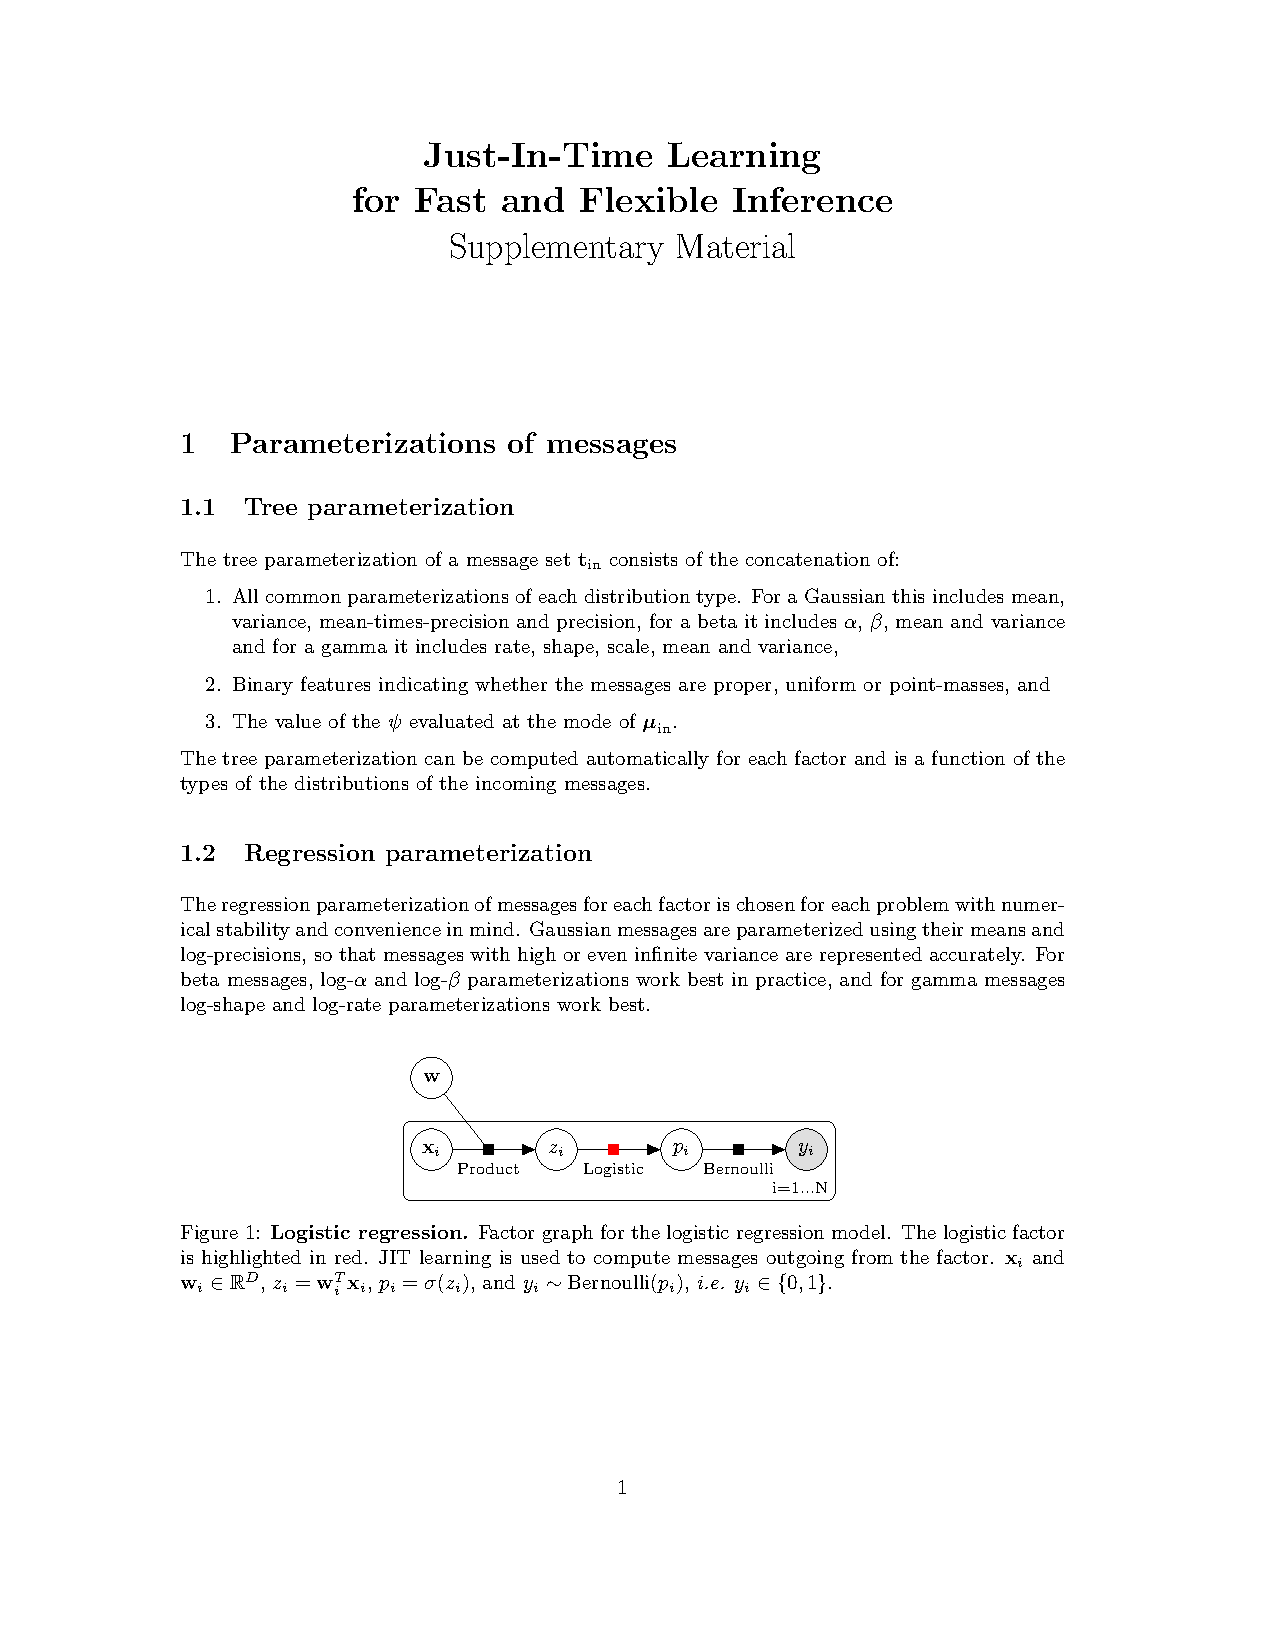
\includegraphics[scale=0.8,page=1,clip,trim=6.5cm 7.5cm 7cm 17.8cm]{img/eslami_jit_supp.pdf}
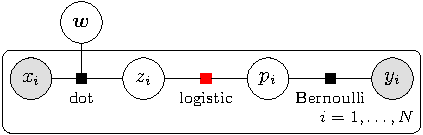
\includegraphics[width=0.8\columnwidth]{binary_logistic_regression-crop}
% \begin{tikzpicture}
%  \node[obs] (x) {$x_i$};
%  \bayesfactor[right= of x] {dot} {below:dot} {} {};
%  \node[latent, above = 5mm of dot] (w) {$\boldsymbol{w}$};
%  \node[latent, right = 6mm of dot] (z) {$z_i$};
%  \bayesfactor[right= 6mm of z, color=red] {logistic} {below:logistic} {} {};
%  \node[latent, right = 6mm of logistic] (p) {$p_i$};
%  \bayesfactor[right = 6mm of p] {bern} {below:Bernoulli} {} {};
%  \node[obs, right = 6mm of bern]  (y)   {$y_i$}; %
%  
%  \edge[-] {dot} {x} ;
%  \edge[-] {w} {dot};
%  \edge[-] {dot} {z} ;
%  \edge[-] {z} {logistic} ;
%  \edge[-] {logistic} {p};
%  \edge[-] {p} {y} ;
%  
%   \plate {sample} { %
%     (x)  (z) (p) (y)
%   } {$i=1, \ldots, N$} ;  
% \end{tikzpicture}
\caption{Factor graph for binary logistic regression. 
The kernel-based message operator learns to approximate the logistic factor 
highlighted in red. 
}
\label{fig:factor_graph_binlog}
\end{figure}


% UCI datasets. temporal uncertainty.
\begin{figure*}[t]
\centering
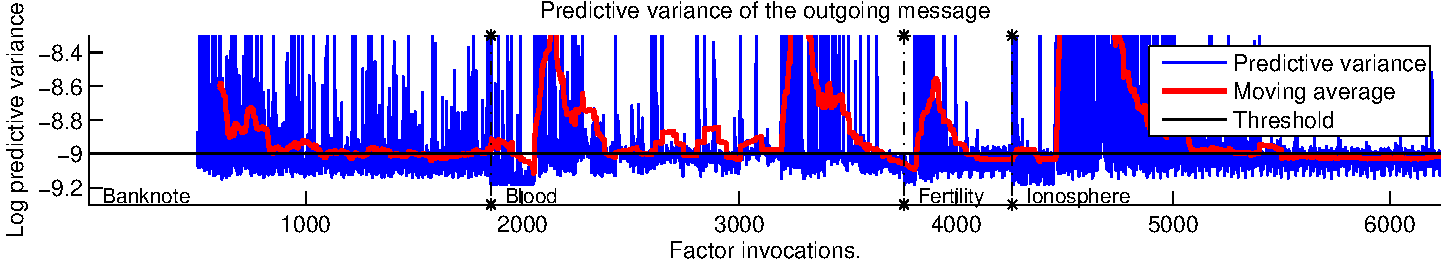
\includegraphics[width=0.95\textwidth]{online/uci_temporal_uncertainty-crop}
\caption{
Uncertainty estimate of KJIT for outgoing messages on the four UCI datasets.
\label{fig:uci_temporal_uncertainty}
}
\end{figure*}


%------------------------------------
%\subsection{Real data}
%------------------------------------


We test the approximate operator in the logistic regression
model as part of the full EP inference loop in a just-in-time learning setting
(KJIT). We used four binary classification datasets from the UCI repository
\citep{Lichm2013}: banknote authentication, blood transfusion, fertility and
ionosphere, in binary logistic regression setting. The
operator was required to learn just-in-time to send outgoing messages
$\msg{\factor}{z_i}$ and $\msg{\factor}{p_i}$ on the four problems presented in
sequence. The training observations consisted of 200 data points subsampled
from each dataset by stratified sampling.  For the fertility dataset, which
contains only 100 data points, we subsampled half the points. The remaining
data were used as test sets. 

We employed a ``minibatch'' idea in which the operator always consults the oracle in
the first few hundred factor invocations for initial batch training. 
In principle, during the initial batch training, the operator can perform 
cross validation or optimizing the marginal likelihood for parameter selection;
however for computational simplicity we set the kernel parameters according to
the median heuristic
\citep{Scholkopf2002}. 
The numbers 
of random features were $D_\mathrm{in} = 300$ and $D_\mathrm{out} = 500$; empirically, we observed
no significant improvements beyond 1,000 random features. The
output noise variance 
$\sigma^2_y$ was fixed to $10^{-4}$ and the uncertainty threshold on the log 
predictive variance (over which the oracle is queried) was set to -9. To
simulate a black-box setup, we used
an importance sampler as the oracle rather than Infer.NET's factor implementation, 
where the proposal distribution was fixed to $\mathcal{N}(z; 0, 200)$ with 
$5 \times 10^5$ particles. We set the
maximum number of EP iterations to 10 in each problem.




% UCI data classification error
% Inference time
\begin{figure}[ht]
  \centering
  \subfloat[Binary classification error\label{fig:uci_01_loss}]{
  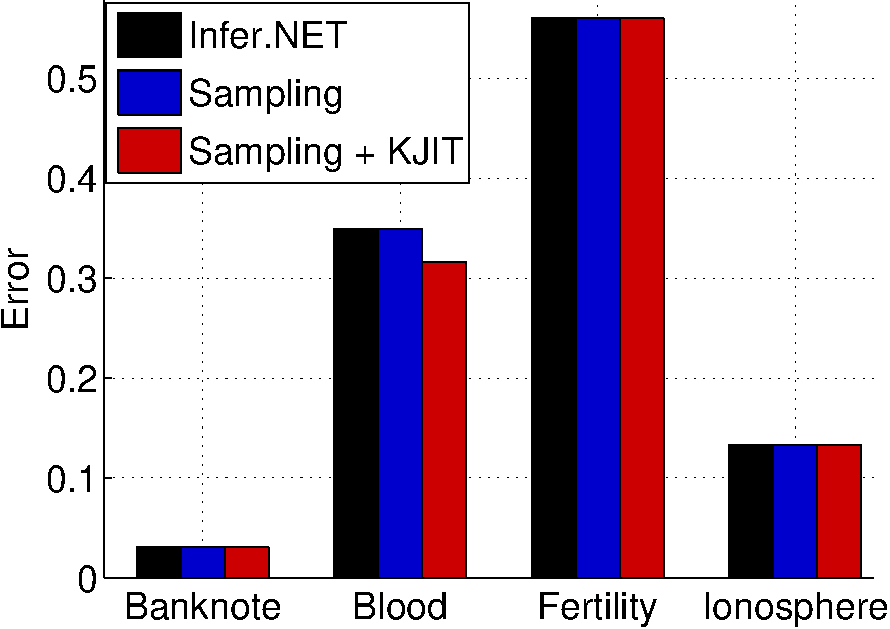
\includegraphics[width=0.49\columnwidth]{online/uci_classification-crop}
  }
  %
  \subfloat[Inference time\label{fig:uci_infer_time}]{
  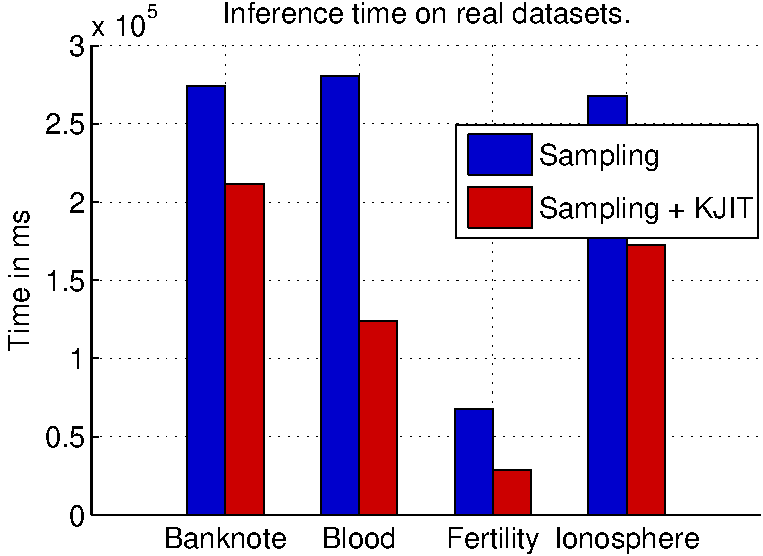
\includegraphics[width=0.49\columnwidth]{online/uci_infer_time-crop}
  }
  \caption{Classification performance and inference times on the four UCI datasets. 
   }
  \label{fig:uci_performance}
\end{figure}


Classification errors on the test sets and inference times are shown in 
\figref{fig:uci_01_loss} and \figref{fig:uci_infer_time}, respectively.
The results demonstrate that KJIT improves the inference time on all the 
problems without sacrificing inference accuracy. The  predictive 
variance of each outgoing message is shown in 
\figref{fig:uci_temporal_uncertainty}. An essential feature to notice is the 
rapid increase of the uncertainty after the first EP iteration of each problem. 
The sharp rise followed by a steady decrease of the uncertainty is a good indicator 
that the operator is able to promptly detect a change in input message distribution,
and robustly adapt to this new distribution by querying the oracle.




\textbf{Experiment 2: Compound gamma factor} We next simulate the compound gamma factor, 
 a heavy-tailed prior distribution on the precision of a Gaussian random variable.
A variable $\tau$ is said to follow the compound gamma distribution 
if $\tau \sim \text{Gamma}(\tau; s_2, r_2)$ (shape-rate parameterization) and 
$r_2 \sim \text{Gamma}(r_2; s_1, r_1)$ where $(s_1, r_1, s_2)$ are parameters. 
The task we consider is to infer the posterior of the precision $\tau$ of a normally 
distributed variable $x \sim \mathcal{N}(x; 0, \tau)$ given realizations 
$\{x_i\}_{i=1}^n$. We consider the setting $(s_1, r_1, s_2) = (1, 1, 1)$ which was 
used in \cite{Heess2013}. Infer.NET's implementation requires two gamma factors
to specify the compound gamma. Here, we collapse them into one factor 
and let the operator learn to directly send an outgoing message $\msg{\factor}{\tau}$ 
given $\msg{\tau}{\factor}$, using Infer.NET as the oracle. 
The  default implementation of Infer.NET relies on a quadrature method.
As in \cite{Eslami2014}, we sequentially presented a number of 
problems to our algorithm, where at the beginning of each problem, a random number of observations 
from 10 to 100, and the parameter $\tau$, were drawn from the model.

% compound gamma inferred results and time.
\begin{figure}[ht]
  \centering
% 	\subfloat[Posteriors]{
% 	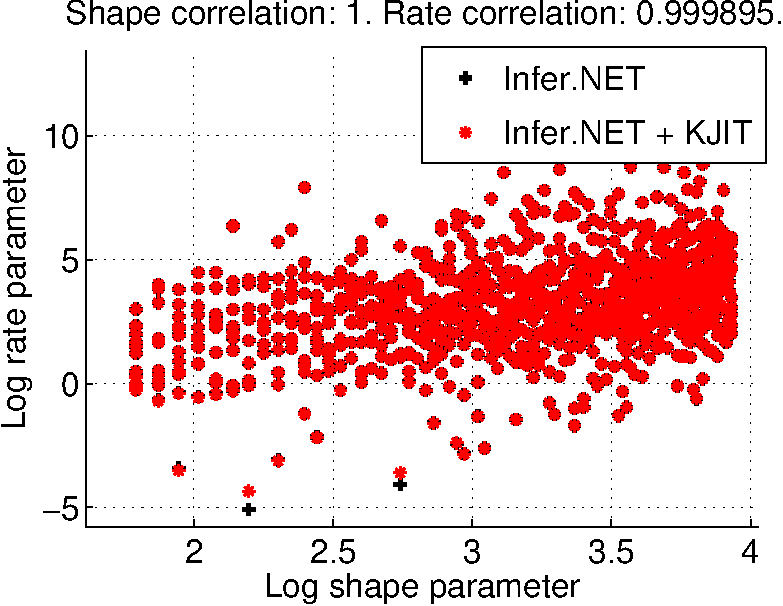
\includegraphics[width=0.49\columnwidth]{img/online/cg_post_corr-crop}
% 	%\missingfigure[figwidth=0.49\columnwidth]{}
% 	}
  %
  \subfloat[Inferred shape \label{fig:cg_infer_shape}]{
  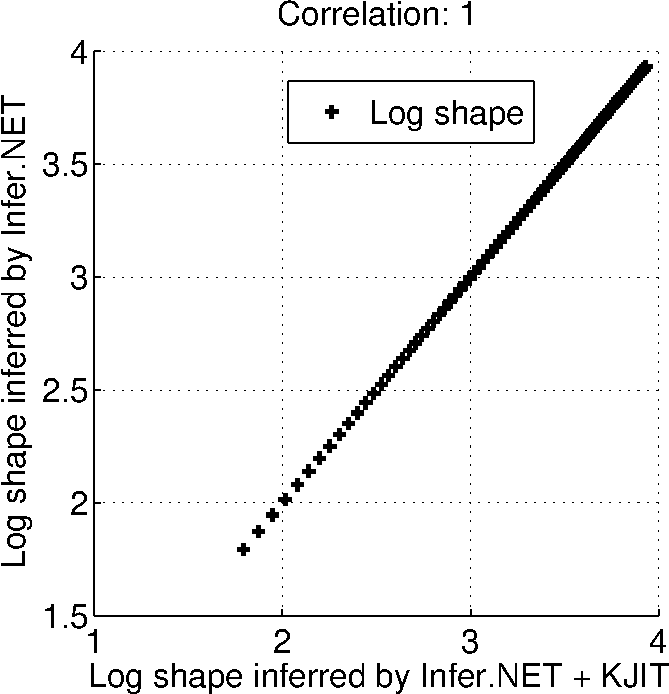
\includegraphics[width=0.33\columnwidth]{online/cg_post_shape-crop}
  %\missingfigure[figwidth=0.49\columnwidth]{}
  }
  %
  \subfloat[Inferred rate \label{fig:cg_infer_rate}]{
  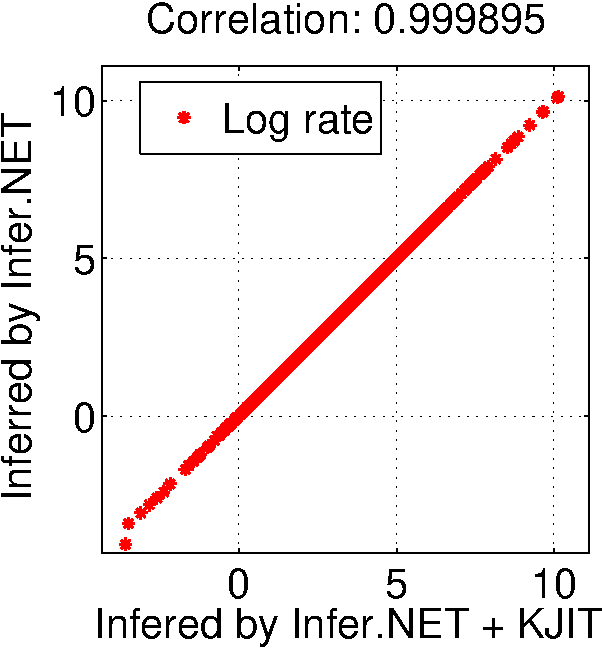
\includegraphics[width=0.31\columnwidth ]{online/cg_post_rate-crop}
  %\missingfigure[figwidth=0.49\columnwidth]{}
  }
  %
  \subfloat[Inference time\label{fig:cg_infer_time}]{
  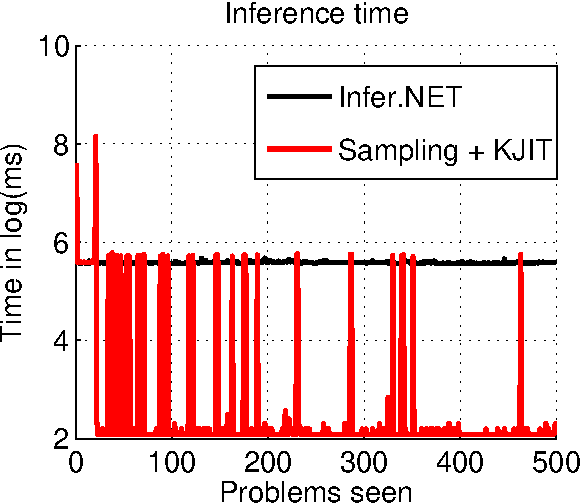
\includegraphics[width=0.33\columnwidth]{online/cg_inference_time-crop}
  }
  \caption{Shape (a) and rate (b) parameters of the inferred posteriors in 
  the compound gamma problem. 
  (c) KJIT is able to infer equally good posterior parameters compared to Infer.NET 
  while requiring a runtime several orders of magnitude lower. }
  \label{fig:cg_performance}
\end{figure}

\figref{fig:cg_infer_shape} and \figref{fig:cg_infer_rate} summarize the inferred 
posterior parameters obtained from running only Infer.NET and Infer.NET + KJIT, i.e., 
KJIT with Infer.NET as the oracle. \figref{fig:cg_infer_time} shows the inference 
time of both methods. The plots collectively show that KJIT can deliver posteriors 
in good agreement with those obtained from Infer.NET, at a much lower cost. 
Note that in this task only one message is passed to the factor in each problem.
\figref{fig:cg_infer_time} also indicates that KJIT requires fewer oracle 
consultations as more problems are seen.
%\subsection*{Acknowledgement}
%Gatsby Charitable Foundation for funding.

%=============================================
\section{Conclusions and future work\label{sec:Conclusions-and-Future} }
%=============================================

We have proposed a method for learning the mapping between incoming and outgoing
messages to a factor in expectation propagation, which can be used
in place of computationally demanding Monte Carlo estimates of these updates.
Our operator has two main advantages: it can reliably evaluate the uncertainty of its prediction,
so that it only consults a more expensive oracle when it is uncertain,
and it can efficiently update its mapping online, so that it learns
from these additional consultations. Once trained, the learned mapping
performs as well as the oracle mapping, but at a far lower computational cost.
This is in large part due to a novel two-stage random feature representation of the input
messages. One topic of current research is hyperparameter selection:
at present, these are learned on an initial mini-batch of data, however
a better option would be to adapt them online as more data are seen.



%% In this work, we made one step forward toward the goal of having a fully 
%% automatic and fast inference engine. 
%% We demonstrated that inference with EP can be sped up without 
%% losing inference accuracy by embedding an uncertainty aware distribution-to-distribution 
%% regressor at a factor node for sending outgoing EP messages given incoming messages.
%% The regressor essentially acts as a cache for message computation, offering 
%% the factor an outgoing message when it is certain about an input. 
%% The proposed use kernel ridge regression 
%% in the primal form with random feature representation of incoming messages 
%% leads to a number of desirable properties for JIT learning: powerful 
%% representation of incoming messages, ease of online update and efficient outgoing 
%% message computation. 
%% Nonetheless, the random feature map itself depends on 
%% hyperparameters which may need to be adapted during inference.
%% Our future works will address this issue. 

%In effect, computing an outgoing message
%amounts to computing the moment parameters by multiplying the ramdom feature vector
%with a matrix given by the solution of the regression.

%Ali's email summary below:
%Hassle-free Bayesian inference is increasingly popular. Some people have been using learned message passing operators for this. However we don't want to have to train the operators in advance (since we'd have to guess input messages). To avoid this, we have to do JIT learning. To do this, we need fast updates and uncertainty. Eslami et al. do this but their method is unprincipled and slow. KJIT addresses both issues.



%\pagebreak
% {\small 
\bibliographystyle{abbrvnat}
\bibliography{../uai2015/ref}
% }


\end{document}
